\documentclass[ignorenonframetext,aspectratio=169,dvipsnames]{beamer}
\setbeamertemplate{caption}[numbered]
\setbeamertemplate{caption label separator}{: }
\setbeamercolor{caption name}{fg=normal text.fg}
\beamertemplatenavigationsymbolsempty
\usepackage{lmodern}
\usepackage{amssymb,amsmath}
\usepackage{ifxetex,ifluatex}
\usepackage{fixltx2e} % provides \textsubscript
\ifnum 0\ifxetex 1\fi\ifluatex 1\fi=0 % if pdftex
  \usepackage[T1]{fontenc}
  \usepackage[utf8]{inputenc}
\else % if luatex or xelatex
  \ifxetex
    \usepackage{mathspec}
  \else
    \usepackage{fontspec}
  \fi
  \defaultfontfeatures{Ligatures=TeX,Scale=MatchLowercase}
\fi
% use upquote if available, for straight quotes in verbatim environments
\IfFileExists{upquote.sty}{\usepackage{upquote}}{}
% use microtype if available
\IfFileExists{microtype.sty}{%
\usepackage{microtype}
\UseMicrotypeSet[protrusion]{basicmath} % disable protrusion for tt fonts
}{}
\newif\ifbibliography
\usepackage{color}
\usepackage{fancyvrb}
\newcommand{\VerbBar}{|}
\newcommand{\VERB}{\Verb[commandchars=\\\{\}]}
\DefineVerbatimEnvironment{Highlighting}{Verbatim}{commandchars=\\\{\}}
% Add ',fontsize=\small' for more characters per line
\newenvironment{Shaded}{}{}
\newcommand{\KeywordTok}[1]{\textcolor[rgb]{0.00,0.44,0.13}{\textbf{{#1}}}}
\newcommand{\DataTypeTok}[1]{\textcolor[rgb]{0.56,0.13,0.00}{{#1}}}
\newcommand{\DecValTok}[1]{\textcolor[rgb]{0.25,0.63,0.44}{{#1}}}
\newcommand{\BaseNTok}[1]{\textcolor[rgb]{0.25,0.63,0.44}{{#1}}}
\newcommand{\FloatTok}[1]{\textcolor[rgb]{0.25,0.63,0.44}{{#1}}}
\newcommand{\ConstantTok}[1]{\textcolor[rgb]{0.53,0.00,0.00}{{#1}}}
\newcommand{\CharTok}[1]{\textcolor[rgb]{0.25,0.44,0.63}{{#1}}}
\newcommand{\SpecialCharTok}[1]{\textcolor[rgb]{0.25,0.44,0.63}{{#1}}}
\newcommand{\StringTok}[1]{\textcolor[rgb]{0.25,0.44,0.63}{{#1}}}
\newcommand{\VerbatimStringTok}[1]{\textcolor[rgb]{0.25,0.44,0.63}{{#1}}}
\newcommand{\SpecialStringTok}[1]{\textcolor[rgb]{0.73,0.40,0.53}{{#1}}}
\newcommand{\ImportTok}[1]{{#1}}
\newcommand{\CommentTok}[1]{\textcolor[rgb]{0.38,0.63,0.69}{\textit{{#1}}}}
\newcommand{\DocumentationTok}[1]{\textcolor[rgb]{0.73,0.13,0.13}{\textit{{#1}}}}
\newcommand{\AnnotationTok}[1]{\textcolor[rgb]{0.38,0.63,0.69}{\textbf{\textit{{#1}}}}}
\newcommand{\CommentVarTok}[1]{\textcolor[rgb]{0.38,0.63,0.69}{\textbf{\textit{{#1}}}}}
\newcommand{\OtherTok}[1]{\textcolor[rgb]{0.00,0.44,0.13}{{#1}}}
\newcommand{\FunctionTok}[1]{\textcolor[rgb]{0.02,0.16,0.49}{{#1}}}
\newcommand{\VariableTok}[1]{\textcolor[rgb]{0.10,0.09,0.49}{{#1}}}
\newcommand{\ControlFlowTok}[1]{\textcolor[rgb]{0.00,0.44,0.13}{\textbf{{#1}}}}
\newcommand{\OperatorTok}[1]{\textcolor[rgb]{0.40,0.40,0.40}{{#1}}}
\newcommand{\BuiltInTok}[1]{{#1}}
\newcommand{\ExtensionTok}[1]{{#1}}
\newcommand{\PreprocessorTok}[1]{\textcolor[rgb]{0.74,0.48,0.00}{{#1}}}
\newcommand{\AttributeTok}[1]{\textcolor[rgb]{0.49,0.56,0.16}{{#1}}}
\newcommand{\RegionMarkerTok}[1]{{#1}}
\newcommand{\InformationTok}[1]{\textcolor[rgb]{0.38,0.63,0.69}{\textbf{\textit{{#1}}}}}
\newcommand{\WarningTok}[1]{\textcolor[rgb]{0.38,0.63,0.69}{\textbf{\textit{{#1}}}}}
\newcommand{\AlertTok}[1]{\textcolor[rgb]{1.00,0.00,0.00}{\textbf{{#1}}}}
\newcommand{\ErrorTok}[1]{\textcolor[rgb]{1.00,0.00,0.00}{\textbf{{#1}}}}
\newcommand{\NormalTok}[1]{{#1}}

\usepackage{graphicx,grffile}
\makeatletter
\def\maxwidth{\ifdim\Gin@nat@width>\linewidth\linewidth\else\Gin@nat@width\fi}
\def\maxheight{\ifdim\Gin@nat@height>\textheight0.8\textheight\else\Gin@nat@height\fi}
\makeatother
% Scale images if necessary, so that they will not overflow the page
% margins by default, and it is still possible to overwrite the defaults
% using explicit options in \includegraphics[width, height, ...]{}
%\setkeys{Gin}{width=\maxwidth,height=\maxheight,keepaspectratio}
\newcommand{\includegraphicsscaled}[1]{
    \includegraphics[width=\maxwidth,height=\maxheight,keepaspectratio]{#1}
}

% Prevent slide breaks in the middle of a paragraph:
\widowpenalties 1 10000
\raggedbottom

\AtBeginPart{
  \let\insertpartnumber\relax
  \let\partname\relax
  \frame{\partpage}
}
\AtBeginSection{
  \ifbibliography
  \else
    \let\insertsectionnumber\relax
    \let\sectionname\relax
    \frame{\sectionpage}
  \fi
}
\AtBeginSubsection{
  \let\insertsubsectionnumber\relax
  \let\subsectionname\relax
  \frame{\subsectionpage}
}

\setlength{\parindent}{0pt}
\setlength{\parskip}{6pt plus 2pt minus 1pt}
\setlength{\emergencystretch}{3em}  % prevent overfull lines
\providecommand{\tightlist}{%
  \setlength{\itemsep}{0pt}\setlength{\parskip}{0pt}}
\setcounter{secnumdepth}{0}
\DeclareUnicodeCharacter{00A0}{~}
\DeclareUnicodeCharacter{03B4}{$\delta$}
\DeclareUnicodeCharacter{03B5}{$\varepsilon$}
\DeclareUnicodeCharacter{03C9}{$\omega$}
\DeclareUnicodeCharacter{2124}{\mathbb{Z}}
\DeclareUnicodeCharacter{2193}{$\downarrow$}
\DeclareUnicodeCharacter{2208}{$\in$}
\DeclareUnicodeCharacter{2209}{$\notin$}
\DeclareUnicodeCharacter{220B}{$\ni$}
\DeclareUnicodeCharacter{2227}{$\wedge$}
\DeclareUnicodeCharacter{2228}{$\vee$}
\DeclareUnicodeCharacter{2234}{$\therefore$}
\DeclareUnicodeCharacter{2264}{$\leq$}
\DeclareUnicodeCharacter{2265}{$\geq$}
\DeclareUnicodeCharacter{2605}{$\star$}
\DeclareUnicodeCharacter{1D53D}{\mathbb{F}}

\usefonttheme[onlymath]{serif}
\hypersetup{breaklinks=true,colorlinks,linkcolor=,urlcolor=purple}
\setbeamertemplate{navigation symbols}{}
\setbeamercolor{footnote mark}{fg=gray}
\setbeamerfont{footnote}{size=\tiny}
\usepackage[normalem]{ulem}
\usepackage{listings}
\lstset{
    literate={ }{{~}}1,
    basicstyle=\ttfamily\large,
    keywordstyle=\color{blue}\bfseries,
    commentstyle=\color[rgb]{0,0.5,0}\bfseries\em,
    stringstyle=\color{BrickRed}\bfseries\em
}

\newcommand\greyuline{\bgroup\markoverwith
    {\textcolor{lightgray}{\rule[-0.5ex]{2pt}{0.4pt}}}\ULon}

\title{\Huge \bf Infinite Scroll}
\subtitle{\Large \bf Lazy lists in the Brick TUI library}
\author{\Large \bf Fraser Tweedale\\
    \texttt{@hackuador}}
\date{\large \bf May 15, 2019}

\setbeamertemplate{background}{
  \ifnum\thepage<2%
   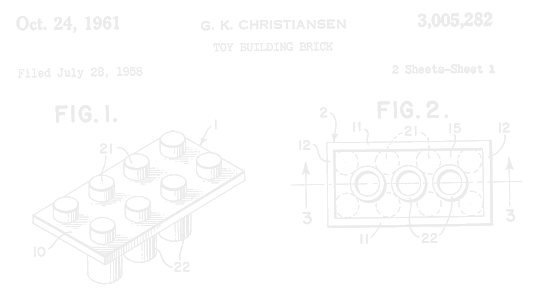
\includegraphics[height=\paperheight,width=\paperwidth]{lego-patent-faded.jpg}
  \fi
}

\begin{document}

\begin{frame}
\titlepage
\end{frame}

\begin{frame}[plain]
\begin{center}
\includegraphicsscaled{../2018-05-22-ylj-ffi/purebred.png}
\end{center}
\end{frame}

\begin{frame}[plain]
\begin{center}
\includegraphicsscaled{brick-final-whitebg.png}
\end{center}
\end{frame}

\begin{frame}[plain]
\huge
  Demo: basic Brick list
\end{frame}

\begin{frame}[fragile]{{\tt Brick.Widget.List} API}
\begin{lstlisting}[language=Haskell]
data List n e

list :: k -> Vector e -> Int -> List n e

listMoveTo :: Int -> List n e -> List n e
listMoveBy :: Int -> List n e -> List n e

listInsert :: Int -> e -> List n e -> List n e
listRemove :: Int ->      List n e -> List n e
\end{lstlisting}
\end{frame}

\begin{frame}[fragile]{{\tt Brick.Widget.List} internals}
\begin{lstlisting}[language=Haskell]
data List n e = List
  { listElements :: Vector e
  , listSelected :: Maybe Int
  , listName :: n
  , listItemHeight :: Int
  }
  deriving (Functor, Foldable, Traversable)

listElementsL :: Lens' (List n e) (Vector e)
listSelectedL :: Lens' (List n e) (Maybe Int)
\end{lstlisting}
\end{frame}

\begin{frame}[plain]
\huge
  Demo: Purebred thread list
\end{frame}

\begin{frame}{Can we lazily load items?}
    \begin{itemize}
        \item Only need to evaluate list up to displayed items
        \item<+-> {\tt Vector} is strict...
        \item<+-> but not all container types are!  % TODO reveal
    \end{itemize}
\end{frame}


\begin{frame}{The plan}  % TODO reveal?
    \begin{enumerate}
        \item Engage upstream
        \item Ensure adequate regression tests
        \item Implementation
    \end{enumerate}
\end{frame}


\begin{frame}[fragile]{Regression tests}
\begin{lstlisting}[language=Haskell]
prop_insertSize :: (Eq a) => Int -> a -> List n a -> Bool
prop_insertSize i a l =
  length (listInsert i a l ^. listElementsL)
    == length (l ^. listElementsL) + 1

prop_insert :: (Eq a) => Int -> a -> List n a -> Bool
prop_insert i a l =
  i >= 0 && i <= length (l ^. listElementsL) ==>
    listSelectedElement (listMoveTo i (listInsert i a l)
    == Just (i, a)
\end{lstlisting}
\end{frame}

\begin{frame}[fragile]{Regression tests}
\begin{lstlisting}[language=Haskell]
data ListMoveOp a
  = MoveUp
  | MoveDown
  | MoveBy Int
  | MoveTo Int
  | MoveToElement a

data ListOp a
  = Insert Int a
  | Remove Int
  | Replace Int [a]
  | Clear
  | ListMoveOp (ListMoveOp a)
\end{lstlisting}
\end{frame}

\begin{frame}[fragile]{Regression tests}
\begin{lstlisting}[language=Haskell]
prop_listOpsMaintainValidSelection
  :: (Eq a) => [ListOp a] -> List n a -> Bool

prop_moveUpReachesBeginning
  :: (Eq a) => [ListOp a] -> List n a -> Bool
\end{lstlisting}
\end{frame}

\begin{frame}[fragile]{Implementation (before)}
\begin{lstlisting}[language=Haskell]
data List n e = List
  { listElements :: Vector e
  , listSelected :: Maybe Int
  , listName :: n
  , listItemHeight :: Int
  }
  deriving (Functor, Foldable, Traversable)

 
\end{lstlisting}  % FIXME NBSP to align with next slide
\end{frame}

\begin{frame}[fragile]{Implementation (after)}
\begin{lstlisting}[language=Haskell]
data GenericList n t e = List
  { listElements :: t e
  , listSelected :: Maybe Int
  , listName :: n
  , listItemHeight :: Int
  }
  deriving (Functor, Foldable, Traversable)

type List n e = GenericList n Vector e
\end{lstlisting}
\end{frame}

\begin{frame}[fragile]{Implementation (after)}
\begin{lstlisting}[language=Haskell]
class Splittable t where
    {-# MINIMAL splitAt #-}

    -- Equivalent to '(take n xs, drop n xs)'
    splitAt :: Int -> t a -> (t a, t a)

    -- Equivalent to '(take n . drop i) xs'
    slice :: Int -> Int -> t a -> t a
    slice i n = fst . splitAt n . snd . splitAt i

instance Splittable Vector where
  -- | /O(1)/
  splitAt = Data.Vector.splitAt
\end{lstlisting}
\end{frame}

\begin{frame}[fragile]{Implementation (before)}
\begin{lstlisting}[language=Haskell]
listMoveTo
  :: ()
  => Int -> List n e -> List n e
listMoveTo pos l =
  let
    len = length l
    i = if pos < 0 then len - pos else pos
  in
    l & listSelectedL .~ if null l
          then Nothing
          else Just $ clamp 0 (len - 1) i
\end{lstlisting}
\end{frame}

\begin{frame}[fragile]{Implementation (after)}
\begin{lstlisting}[language=Haskell]
listMoveTo
  :: (Foldable t, Splittable t)
  => Int -> GenericList n t e -> GenericList n t e
listMoveTo pos l =
  let
    len = length l
    i = if pos < 0 then len - pos else pos
  in
    l & listSelectedL .~ if null l
          then Nothing
          else Just $ splitClamp l i
\end{lstlisting}
\end{frame}

\begin{frame}[fragile]{Implementation (before/after)}
\begin{lstlisting}[language=Haskell]
clamp :: (Ord a) => a -> a -> a -> a
clamp lo hi = max lo . min hi

splitClamp
  :: (Foldable t, Splittable t)
  => GenericList n t e -> Int -> Int
splitClamp l i =
  let (_, t) = splitAt i (l ^. listElementsL)
  in clamp 0 (if null t then length l - 1 else i) i
\end{lstlisting}
\end{frame}
% if:
% - structure itself is lazy;
% - and splitAt does not evaluate tail;
% - and index is non-negative (negative counts from back)
% - THEN listMoveTo will not force the "rest of structure"

\begin{frame}[fragile]{\tt Data.Sequence.Seq}
\begin{lstlisting}[language=Haskell]
instance Splittable Seq where
  -- | /O(log(min(i,n-1)))/
  splitAt = Data.Sequence.splitAt
\end{lstlisting}
\end{frame}

\begin{frame}[fragile]{Testing laziness}
\begin{lstlisting}[language=Haskell]
newtype L a = L [a]
  deriving (Functor, Foldable)

instance Splittable L where ...

prop_moveByPosLazy :: Bool
prop_moveByPosLazy =
  let
    v = L (1:2:3:4:undefined) :: L Int
    l = list () v 1  -- initial selection is 0
    l' = listMoveBy 1 l
  in
    l' ^. listSelectedL == Just 1  -- now it's 1
\end{lstlisting}
\end{frame}

\begin{frame}[fragile]{Parametricity}
\begin{lstlisting}[language=Haskell]
-- before
listMoveBy
  :: Int -> List n e -> List n e  -- Vector-based

-- after
listMoveBy
  :: (Foldable t, Splittable t)
  => Int -> GenericList n t e -> GenericList n t e
\end{lstlisting}
\end{frame}

% What is the benefit here?
%
% - the list must be a single slice of the input list
% - elements cannot be reordered

\begin{frame}[plain]
\begin{center}
\def\svgwidth{0.2\textwidth}
\input{purebred-logo-ARTIFACT.pdf_tex}
\end{center}
\end{frame}

\begin{frame}[fragile]{\tt Purebred.LazyVector}
\begin{lstlisting}[language=Haskell]
newtype V a = V [Vector a]  -- linked list of chunks
  deriving (Functor, Foldable, Show)

fromList :: Int -> [a] -> V a
fromList chunkSize xs = ...  -- one chunk at a time

-- | O(n/c).  May fragment a chunk.
instance Splittable V where
  splitAt = ... -- might split chunks

-- Eq and Ord ignore chunk boundaries
-- Semigroup and Monoid (<>) do not defragment chunks
\end{lstlisting}
\end{frame}

\begin{frame}[fragile]{Searching for threads}
\begin{lstlisting}[language=Haskell]
getThreads
  :: (MonadError Error m, MonadIO m)
  => Notmuch.SearchTerm -> FilePath -> m (V Thread)
getThreads query dbPath =
  withDatabaseReadOnly dbPath $
    flip Notmuch.query query
    >=> Notmuch.threads  -- thread list produced lazily
    >=> liftIO . lazyTraverse processThread
    >=> pure . fromList 128 -- chunk size

lazyTraverse :: (a -> IO b) -> [a] -> IO [b]
lazyTraverse f = foldr
  (\x ys -> (:) <$> f x <*> unsafeInterleaveIO ys)
  (pure [])
\end{lstlisting}
\end{frame}

\begin{frame}[plain]
\huge
  Demo: Purebred lazy list
\end{frame}

\begin{frame}[fragile]{List size notification}
\begin{lstlisting}[language=Haskell]
-- compute length in background; emit notification
notifyNumThreads
  :: (Foldable t)
  => BChan PurebredEvent -> t a -> IO ()
notifyNumThreads chan l =
  let
    len = length l
    go = len `seq` writeBChan chan (NotifyNumThreads len)
  in
    forkIO go
\end{lstlisting}
\end{frame}

\begin{frame}[plain]
\huge
  Demo: Background length compute
\end{frame}


\section{\fontsize{64pt}{64pt}\selectfont $\infty$}
% INFINITE SCROLL

% - brick List references head of the structure
% - infinite [] or other lazy type will grow forever (OOM)
%   - unless there's a cyclic reference!
% - otherwise you have to "prune" the list yourself

\begin{frame}[fragile]{Infinite scroll - prune list}
\begin{lstlisting}[language=Haskell]
pruneList
  :: (L.Splittable t)
  => L.GenericList n t a -> L.GenericList n t a
pruneList l =
  case l ^. L.listSelectedL of
    Nothing -> l
    Just i ->
      let
        i' = max 0 (i - 999)
      in
        ($l) $
          over L.listElementsL (snd . L.splitAt i')
          . set L.listSelectedL (Just (i - i'))
\end{lstlisting}
\end{frame}

\begin{frame}[fragile]{Infinite scroll - prune list}
\begin{lstlisting}[language=Haskell]
appEvent
  :: L.GenericList () L Int
  -> T.BrickEvent () e
  -> T.EventM () (T.Next (L.GenericList () L Int))
appEvent l ev = case ev of
  T.VtyEvent (V.EvKey V.KEsc []) -> M.halt l
  T.VtyEvent vev ->
    M.continue . pruneList =<< L.handleListEvent vev l
  _ -> M.continue l
\end{lstlisting}
\end{frame}

\begin{frame}[plain]
\huge
  Demo: Infinite scroll
\end{frame}


\begin{frame}[plain]
\begin{columns}

  \begin{column}{.4\textwidth}
    \begin{center}
    {
        \Large Questions?\\
        \medskip
        \includegraphicsscaled{brick-final-whitebg.png}
    }
    \end{center}


  \end{column}

  \begin{column}{.6\textwidth}
    \hypersetup{urlcolor=black}

    \setlength{\parskip}{.5em}

    { \centering

    \input{cc-by-ARTIFACT.pdf_tex}
    \\
    { \scriptsize
    Except where otherwise noted this work is licensed under
    }\\
    { \footnotesize
      \textbf{\url{http://creativecommons.org/licenses/by/4.0/}}
    }

    \bigskip
    \large \tt

    \url{https://speakerdeck.com/frasertweedale}

    \href{https://twitter.com/hackuador}{@hackuador}

    \href{https://github.com/jtdaugherty/brick}{jtdaugherty/brick}

    \href{https://github.com/purebred-mua/purebred}{purebred-mua/purebred}

    }
  \end{column}

\end{columns}
\end{frame}

\end{document}
